% 2008 年重庆卷理科第 19 题：△ABC（B=90°）中 D∈AB、E∈AC，AD/DB=AE/EC=2，DE=3，
%   沿 DE 折成直二面角。
% 来源 PDF：gaokaomath-src/普通高考/2008/2008重庆理.pdf
% SHA-256：d3ca36cef73a00068b9c1a97ddb2f90bbc4f16b38459e380579090a02706d937
% 原页：2008重庆理.pdf 第 1 页（A3 三栏）第 3 栏，书页码 429。
% 绘制依据：左图为折叠前的直角三角形（DE ∥ BC），右图为折起后的立体图（虚线为折前的 DE 与 BC 位置）。
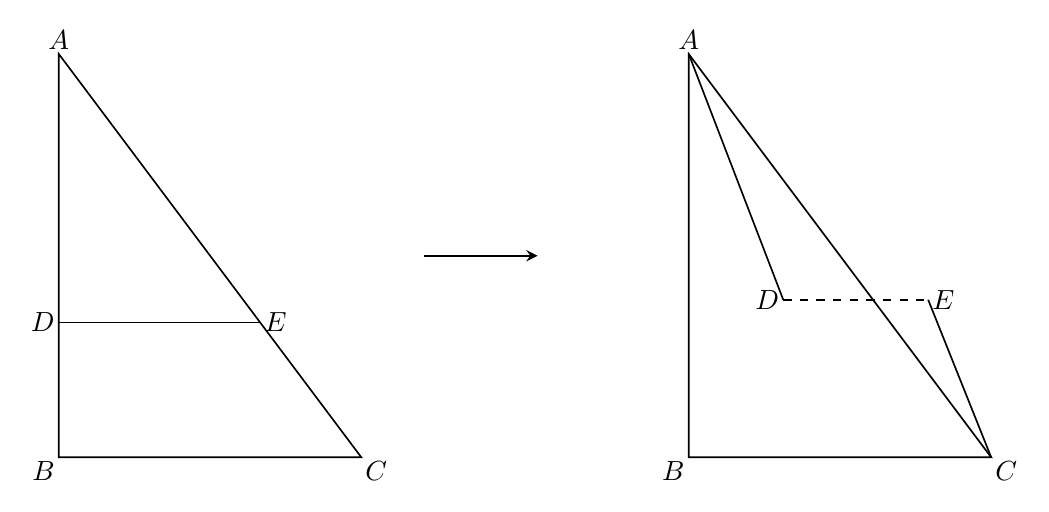
\begin{tikzpicture}[scale=1.6, semithick, every node/.style={inner sep=1.2pt}]
  % 左：折叠前
  \begin{scope}[shift={(0,0)}]
    \coordinate (B) at (0,0);
    \coordinate (C) at (2.4,0);
    \coordinate (A) at (0,3.2);
    \coordinate (D) at (0,1.07);
    \coordinate (E) at (1.6,1.07);
    \draw (A) -- (B) -- (C) -- cycle;
    \draw (D) -- (E);
    \node[below left] at (B) {$B$};
    \node[below right] at (C) {$C$};
    \node[above] at (A) {$A$};
    \node[left] at (D) {$D$};
    \node[right] at (E) {$E$};
  \end{scope}
  % 箭头
  \draw[->,>=stealth, line width=0.8pt] (2.9,1.6) -- (3.8,1.6);
  % 右：折起后
  \begin{scope}[shift={(5.0,0)}]
    \coordinate (B2) at (0,0);
    \coordinate (C2) at (2.4,0);
    \coordinate (A2) at (0,3.2);
    \coordinate (D2) at (0.75,1.25);
    \coordinate (E2) at (1.9,1.25);
    \draw (A2) -- (B2) -- (C2) -- cycle;
    \draw (A2) -- (D2);
    \draw[dashed] (D2) -- (E2);
    \draw (C2) -- (E2);
    \node[below left] at (B2) {$B$};
    \node[below right] at (C2) {$C$};
    \node[above] at (A2) {$A$};
    \node[left] at (D2) {$D$};
    \node[right] at (E2) {$E$};
  \end{scope}
\end{tikzpicture}
